%%%%%%%%%%%%%%%%%%%%%%%%%%%%%%%%%%%%%%%%%%%%%%%%%%%%%%%%%%%%%%%%%%%%%%%%%%%%%%
% Detta �r ett exempel p� ett latexdokument.
% 
% Alla dokument best�r av f�ljande delar:
%
%          \documentclass[optioner]{dokumentklass}
%            ...inst�llningar...
%          \begin{document}
%            ...text...
%          \end{document}
%
% Som ni kanske redan har f�rst�tt �r anv�nds procent (%) f�r
% kommentarer.
%%%%%%%%%%%%%%%%%%%%%%%%%%%%%%%%%%%%%%%%%%%%%%%%%%%%%%%%%%%%%%%%%%%%%%%%%%%%%%

\documentclass[a4paper]{article}

\usepackage{graphicx}
\usepackage{listings}
%\usepackage[T1]{fontenc}                % F�r svenska bokst�ver
%\usepackage[swedish]{babel}             % F�r svensk avstavning och svenska
                                        % rubriker (t ex "inneh�llsf�rteckning)
\title{Programming Project, Database Technology}
\author{Tim Dolck dat11tdo@student.lu.se \\ 
Julian Kron� dat11jkr@student.lu.se \\
Christopher Nilsson dat11cni@student.lu.se}
%\date{}           % Blir dagens datum om det utel�mnas

\begin{document}
\lstset{language=SQL}

\maketitle                      % Skriver ut rubriken som vi
                                % deklarerade ovan med \title, \author
                                % och eventuellt \date
\newpage
\section{Introduction}          % Detta kommando g�r en rubrik

\section{Requirements}

\section{Outline}
Our product is built in play framework. It is a web application framework with support for programming in scala. Play also enables us to easy use a model-view-controller modell which we have used. The view section is mostly built up by html-templates. These templates are filled up with data from scala-variables. The model & controller section are both written in scala. 

The product uses jdbc as databasemanager. The controller section of the program has the connection with the database. It handles all the SQL-queries and sends them to the database.

\section{Model}

\begin{figure}[h]
  \centering
  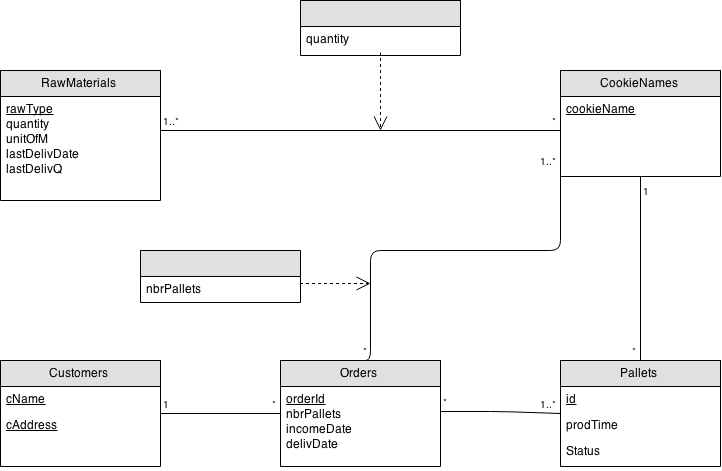
\includegraphics[width=\textwidth]{cookies.png}
  \caption{An UML diagram illustrating the database design.}
  \label{model}
\end{figure}

\section{Statements}

\begin{lstlisting}[frame=single]
--
-- Disable foreign key checks temporarily so 
-- tables can be deleted in arbitrary order, 
-- and so that insertion is faster.

set FOREIGN_KEY_CHECKS = 0;

-- Drop the tables if they already exist.

drop table if exists RawMaterials;
drop table if exists RecipeDetails;
drop table if exists CookieNames;
drop table if exists Pallets;
drop table if exists OrderDetails;
drop table if exists Orders;
drop table if exists Customers;

-- Create the tables.

create table RawMaterials (
    rawType     varchar(30) not null,
    quantity    integer default 100000000 
      check (quantity >= 0),
    unitOfM     enum('g', 'ml') not null,
    lastDeliv   datetime,
    lastDelivQ  integer,
    primary key (rawType)
);

create table RecipeDetails (
    cookieName  varchar(20) not null,
    rawType     varchar(30) not null,
    quantity    integer not null,
    primary key (cookieName, rawType),
    foreign key (cookieName) references 
      CookieNames(cookieName),
    foreign key (rawType) references 
      RawMaterials(rawType)
);

create table CookieNames (
    cookieName  varchar(20) not null,
    primary key (cookieName)
);

create table Pallets (
    id          integer auto_increment,
    prodTime    datetime not null,
    cookieName  varchar(20) not null,
    status      enum('free','blocked','ordered','delivered') 
      not null default 'free',
    orderId     integer default null,
    primary key (id),
    foreign key (cookieName) references 
      CookieNames(cookieName),
    foreign key (orderId) references 
      OrderDetails(orderId)
);

create table Customers (
    cName       varchar(30) not null,
    cAddress    varchar(30) not null,
    primary key (cName, cAddress)
);

create table Orders (
    orderId     integer auto_increment,
    nbrPallets  integer not null check (nbrPallets > 0),
    incomeDate  datetime not null,
    delivDate   datetime not null,
    cName       varchar(30) not null,
    cAddress    varchar(30) not null,
    primary key (orderId),
    foreign key (cName, cAddress) references 
      Customers(cName, cAddress)
);

create table OrderDetails (
    orderId     integer not null,
    cookieName  varchar(20) not null,
    nbrPallets  integer not null check (nbrPallets >= 0),
    primary key (orderId, cookieName),
    foreign key (orderId) references Orders(orderId),
    foreign key (cookieName) references 
      CookieNames(cookieName)
);
\end{lstlisting}


\section{Manual}

\end{document}                 % The input file ends with this command.
